%% ============================================================================
\section{LCS as a Function of \texorpdfstring{$\Lambda$}{Lambda}}
\label{app:lcs-lambda}
%% ============================================================================

The paper states its results for $\Lambda$ (Eq.~\ref{eq:lambda}) and reports $\LCS$
(Eq.~\ref{eq:lcs}). This section gives the map between them. Fix the claim set, the priors and the
committed world, and write $u_0=\pi(\xs)$ and $u=\PR(\xs)$, so that $u=u_0e^{\Lambda}$ by
Eq.~\ref{eq:lambda}; with flat priors, $u_0=2^{-n}$.

\begin{proposition}[$\LCS$ as a function of $\Lambda$]
\label{prop:lcs-lambda}
For a fixed $u_0\in(0,1)$:
\begin{enumerate}[label=(\roman*),leftmargin=1.6em,itemsep=1pt,topsep=2pt]
\item $\Lambda<-\log u_0$; with flat priors, $\Lambda<n\log2$. $\Lambda$ is bounded below for every
  graph, by $\sum_{r\in\Rcon}\log(1-p_r)$, but this bound tends to $-\infty$ as a conflict's weight
  tends to $1$.
\item $\LCS=\frac{e^{\Lambda}(1-u_0)}{1+e^{\Lambda}(1-2u_0)}$, or equivalently
  $\LCS=\sigma\bigl(\Lambda-\log\frac{1-u}{1-u_0}\bigr)$.
\item $\LCS$ is a strictly increasing function of $\Lambda$, with
  $\frac{d\,\LCS}{d\Lambda}=\frac{\LCS(1-\LCS)}{1-u}$, and its inverse is
  $\Lambda=\log\LCS-\log\bigl[(1-\LCS)-u_0(1-2\LCS)\bigr]$.
\item $\LCS=\frac12$ at $\Lambda=0$; $\LCS\to0$ as $\Lambda\to-\infty$, and $\LCS\to1$ as
  $\Lambda\to-\log u_0$, that is, as the relations force $\xs$.
\item $\LCS\ge\sigma(\Lambda)$ for $\Lambda\ge0$ and $\LCS\le\sigma(\Lambda)$ for $\Lambda\le0$,
  with equality only at $\Lambda=0$: $\LCS$ is always at least as far from $\frac12$ as
  $\sigma(\Lambda)$. For a fixed $\Lambda\ne0$, $|\LCS-\sigma(\Lambda)|$ decreases strictly as $u_0$
  decreases, and $\LCS\to\sigma(\Lambda)$ as $u_0\to0$.
\end{enumerate}
\end{proposition}

\paragraph{Proof.}
\begin{itemize}[leftmargin=1.2em,itemsep=1pt,topsep=2pt]
\item[(i)] Every world has positive mass under $\PR$, because priors lie in $(0,1)$ and weights in
  $[0,1)$, so $u<1$ and $\Lambda=\log(u/u_0)<-\log u_0$. The lower bound is
  Prop.~\ref{prop:props}(v).
\item[(ii)] $\operatorname{logit}u-\operatorname{logit}u_0
  =\log\frac{u}{u_0}+\log\frac{1-u_0}{1-u}=\Lambda-\log\frac{1-u}{1-u_0}$, which is the second
  form. For the first, $\sigma(z)=O/(1+O)$ with
  $O=e^z=\frac{u(1-u_0)}{u_0(1-u)}=\frac{e^{\Lambda}(1-u_0)}{1-u_0e^{\Lambda}}$, and
  $1-u_0e^{\Lambda}+e^{\Lambda}(1-u_0)=1+e^{\Lambda}(1-2u_0)$.
\item[(iii)] With $z$ the argument of $\sigma$ in (ii), $\frac{dz}{d\Lambda}
  =1+\frac{u_0e^{\Lambda}}{1-u_0e^{\Lambda}}=\frac1{1-u}>0$ and $\sigma'=\sigma(1-\sigma)$.
  Solving $\LCS\,(1+e^{\Lambda}(1-2u_0))=e^{\Lambda}(1-u_0)$ for $e^{\Lambda}$ gives the inverse.
\item[(iv)] Substitute $\Lambda=0$ in (ii). As $\Lambda\to-\infty$ the numerator tends to $0$.
  As $e^{\Lambda}\to1/u_0$, $\LCS\to\frac{(1-u_0)/u_0}{1+(1-2u_0)/u_0}=1$.
\item[(v)] The correction $\log\frac{1-u_0}{1-u}$ added to $\Lambda$ in (ii) is positive exactly
  when $u>u_0$, that is when $\Lambda>0$, negative when $\Lambda<0$, and zero at $\Lambda=0$, and
  $\sigma$ is strictly increasing. For a fixed $\Lambda$, the correction
  $c(u_0)=\log(1-u_0)-\log(1-u_0e^{\Lambda})$ has
  $c'(u_0)=\frac{e^{\Lambda}-1}{(1-u_0)(1-u_0e^{\Lambda})}$, which has the sign of $\Lambda$, as $c$
  does; so $|c|$ shrinks strictly as $u_0$ falls, and $c\to0$ as $u_0\to0$, because then
  $u=u_0e^{\Lambda}\to0$. $\square$
\end{itemize}

\begin{figure*}[t]
\centering
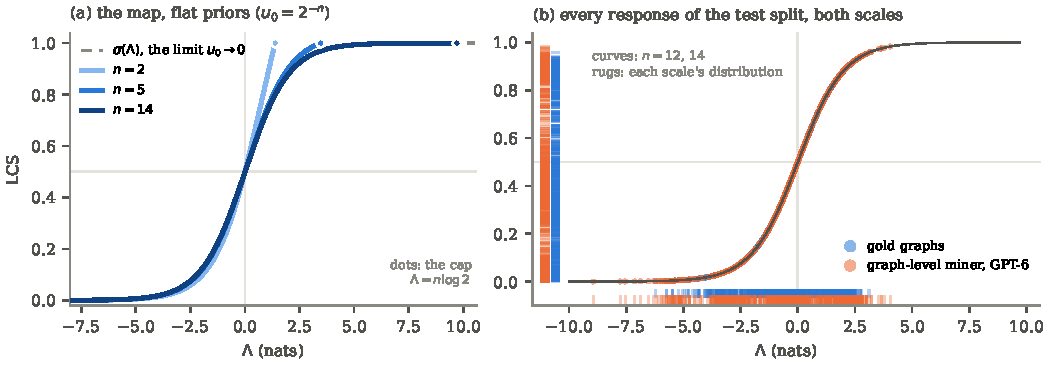
\includegraphics[width=\textwidth]{figures/fig_lcs_lambda.pdf}
\caption{\textbf{$\LCS$ and $\Lambda$.} (a) The map of Prop.~\ref{prop:lcs-lambda} with flat
priors for $n=2$, $5$ and $14$ claims; each curve approaches $\LCS=1$ at its cap $\Lambda=n\log2$
(a supremum that no graph reaches). The dashed line is the limit $\sigma(\Lambda)$; at $n=14$ the curve coincides with it.
(b) Every LoCoBench response as $(\Lambda,\LCS)$, on gold graphs and on the GPT-6 graph-level arm's
graphs, with each scale's distribution as a rug. $\Lambda$ ranges over several nats in either
direction, and $\LCS$ over most of $(0,1)$, compressed near its ends; the points lie on the curves for the
ladders' $12$--$14$ claims.}
\label{fig:lcs-lambda}
\end{figure*}

\paragraph{On the ladders.} Every LoCoBench response has \lclNMin--\lclNMax{} claims and flat
priors, so the cap $n\log2$ lies at \lclLamCapMin--\lclLamCapMax{} nats. The observed values stay
well below it:
\begin{itemize}[leftmargin=1.2em,itemsep=1pt,topsep=2pt]
\item on gold graphs, $\Lambda$ runs from $\lclLamMinGold$ to $\lclLamMaxGold$;
\item on the GPT-6 graph-level arm's graphs, from $\lclLamMinGpt$ to $\lclLamMaxGpt$.
\end{itemize}
So $u$ stays small, the correction in (ii) is negligible, and $\LCS$ equals $\sigma(\Lambda)$ to
within $\lclMaxDevSigma$ on every response (Figure~\ref{fig:lcs-lambda}b). The closed form (ii)
reproduces the scorer on the \lclNGold{} responses of each arm to within $\lclCheckErr$, and the inverse
in (iii) recovers $\Lambda$ to within $\lclInvErr$. On gold graphs \lclLowGold\% of responses, and on
the GPT-6 graph-level arm's \lclLowGpt\%, have $\LCS<0.01$; none exceeds $0.99$.

\paragraph{Why two scales.} By (iii), a step $\Delta$ in $\Lambda$ moves $\LCS$ by about
$\LCS(1-\LCS)\,\Delta/(1-u)$, which is $\LCS(1-\LCS)\,\Delta$ while $u$ is small. Moving $\LCS$ by
$\tau$ therefore takes a step of about $\tau/[\LCS(1-\LCS)]$ nats:
\begin{itemize}[leftmargin=1.2em,itemsep=1pt,topsep=2pt]
\item $0.04$ nats at $\LCS=\frac12$;
\item about one nat at $\LCS=0.01$ or $0.99$;
\item far more than any single relation can supply near $\LCS\approx10^{-17}$.
\end{itemize}
This is why the gold increases that fall below $\tau$ all lie near the ends of the scale, and why
\emph{whether} the score moves is decided on $\Lambda$ while \emph{how far} it moves is read on
$\LCS$ (``One score, two scales'', App.~\ref{app:setup-details}). Since the map is strictly increasing,
the two scales never disagree on the direction of a change.

\paragraph{Additivity and the claim set.} For relations on disjoint sets of claims, $\Lambda$ adds
(Prop.~\ref{prop:props}(iii)), and $u_0$ multiplies. The $\LCS$ of the union is the map (ii) at
$\Lambda_1+\Lambda_2$ with $u_0=u_{0,1}u_{0,2}$, which depends on both claim sets and is not a
function of the two $\LCS$ values alone. Likewise, a claim that no relation touches halves $u_0$
under flat priors and leaves $\Lambda$ unchanged, so by (v) it moves $\LCS$ slightly towards
$\sigma(\Lambda)$. Statements about sums and bounds are therefore made for $\Lambda$.

